% Created 2020-03-11 Wed 20:53
% Intended LaTeX compiler: pdflatex
\documentclass[presentation]{beamer}
\usepackage[utf8]{inputenc}
\usepackage[T1]{fontenc}
\usepackage{graphicx}
\usepackage{grffile}
\usepackage{longtable}
\usepackage{wrapfig}
\usepackage{rotating}
\usepackage[normalem]{ulem}
\usepackage{amsmath}
\usepackage{textcomp}
\usepackage{amssymb}
\usepackage{capt-of}
\usepackage{hyperref}
\usepackage{minted}
\usepackage[T2A]{fontenc}
\usepackage[utf8]{inputenc}
\usepackage[english, russian]{babel}
\usetheme{Frankfurt}
\useinnertheme{rounded}
\author{Макаров Сергей}
\date{\today}
\title{Описание семантики машинных команд для абстрактной интерпретации}
\hypersetup{
 pdfauthor={Макаров Сергей},
 pdftitle={Описание семантики машинных команд для абстрактной интерпретации},
 pdfkeywords={},
 pdfsubject={},
 pdfcreator={Emacs 26.3 (Org mode 9.3)}, 
 pdflang={Russian}}
\begin{document}

\maketitle

\section{Введение}
\label{sec:org67bb2ac}
\begin{frame}[label={sec:orgc6e0dd7}]{Мотивация}
\begin{itemize}
\item В современных решениях для анализа бинарного кода одни и те же задачи, в частности, декодирование команд и трансляция их в промежуточное представление, решаются каждый раз заново, для каждой частной задачи.
\item В рамках проекта Glassfrog предлагается унифицированный подход для решения задач декодирования процессорных команд, трансляции их в промежуточное представление и анализа полученного представления.
\item Для описания форматов файлов, формата и семантики машинных команд предлагается использование внутреннего языка спецификаций с расчётом на то, что поддерживать такие спецификации проще, чем код.
\item В качестве решения для задач анализа кода предлагается подход, основанный на теории абстрактной интерпретации.
\end{itemize}
\end{frame}
\begin{frame}[label={sec:org779437b}]{Glassfrog}
\begin{center}
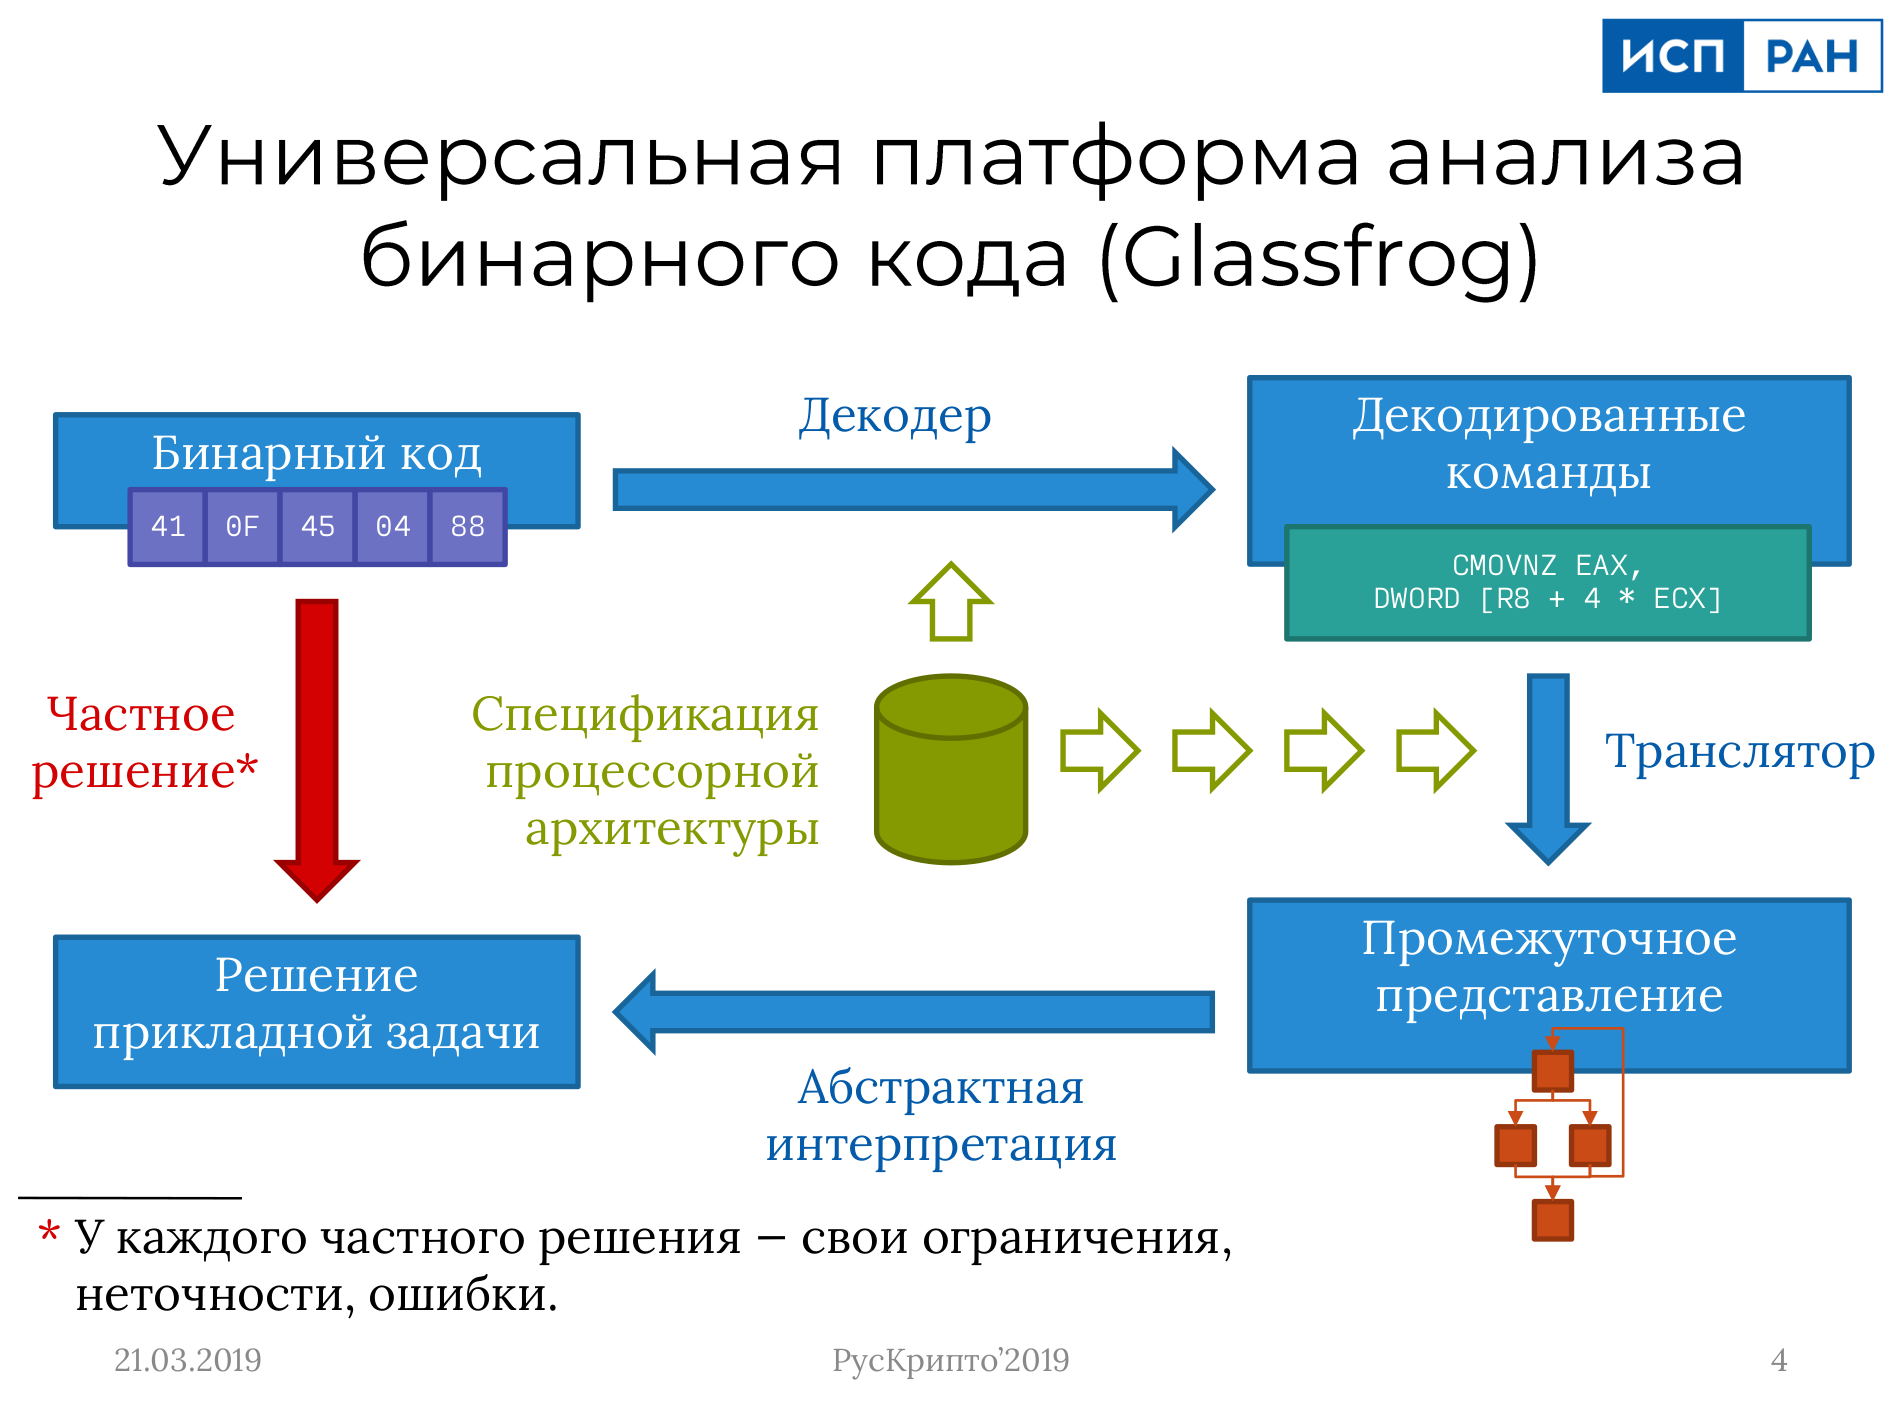
\includegraphics[width=.9\linewidth]{./glassfrog.png}
\end{center}
\end{frame}
\section{Промежуточное представление}
\label{sec:orgaf84483}
\begin{frame}[label={sec:orgfd4929c}]{Pivot 2}
Анализ кода производится над внутренним промежуточным представлением Pivot 2. Рассмотрим
основные структурные элементы этого представления:
\begin{itemize}
\item Адресные пространства
\item Операции
\item Временные переменные
\item Операторы
\item Базовые блоки
\item Фрагменты
\end{itemize}
\end{frame}
\begin{frame}[label={sec:org23ef167},fragile]{Адресные пространства и регистры}
 Адресные пространства описывают память, с которой могут работать команды процессора. Могут
быть локальными или удалёнными. Пример описания адресного пространства:
\begin{minted}[]{text}
space registers: local[u8];
space iomem: remote[i8] ~> i4;
\end{minted}

На уровне спецификаций также есть \alert{регистры} -- ссылки на ячейки адресного пространства
определённого размера:
\begin{minted}[]{text}
register x1: u32 from registers;
\end{minted}
\end{frame}
\begin{frame}[label={sec:org4ea4147},fragile]{Операции}
 Операции принимают на вход набор битовых векторов и возвращают набор битовых векторов. Для
операций должны быть выполнены следующие требования:
\begin{enumerate}
\item Нет побочных эффектов, все входные и выходные данные -- формальные параметры.
\item Все входы влияют на все выходы.
\end{enumerate}
Пример описания операции:
\begin{minted}[]{text}
op add<T: Integer>(a: T, b: T) -> (default result: T,
                                   cf: bool, of: bool)
where
    result = 'add(a, b);
    cf = 'adduo(a, b);
    of = 'addso(a, b);
\end{minted}
\end{frame}
\begin{frame}[label={sec:org1b52cee}]{Базовые блоки}
Базовый блок представляет собой непрерывную с точки зрения потока управления последовательность
операторов. Передача данных между блоками осуществляется посредством групп временных переменных.
Вместо \(\phi\)-функции используется следующий механизм: из каждого блока есть два выхода, "истинный"
и "ложный". Выбор выхода зависит от значения специальной управляющей временной переменной
размера 1. Каждому выходу назначается группа переменных, передаваемых в этом направлении.
Аналогично, для "принимающего" блока задаётся группа входных переменных.
\end{frame}
\begin{frame}[label={sec:org67a68fe}]{Базовые блоки}
Пример графа потока управления, соответствующего простейшему условному переходу:
\begin{center}
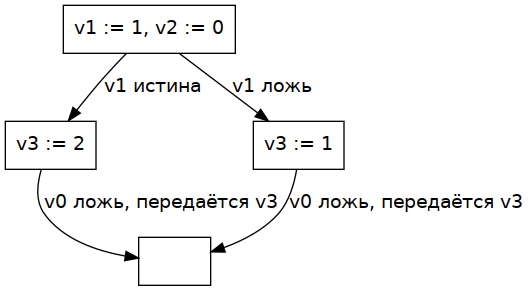
\includegraphics[width=.9\linewidth]{cfg.png}
\end{center}
\end{frame}
\begin{frame}[label={sec:orge13aaed}]{Фрагменты (уровень Pivot 2)}
Фрагмент является самой крупной структурной единицей промежуточного представления. Логически
фрагмент -- это граф, вершинами которого являются базовые блоки, с одним входом и одним выходом.
Входные параметры фрагмента совпадают с входной группой входного блока. Входной блок может
иметь пустую группу входных переменных. Результатом работы фрагмента является
группа временных переменных, возвращаемая выходным блоком.
\end{frame}
\begin{frame}[label={sec:orgd7569ed},fragile]{Функции (уровень спецификаций)}
 Пример спецификации для функции:
\begin{minted}[]{text}
fn g(a: u8, b: u8) -> (result: bits(13))
{
        let result: bits(13) = if <a, b>[0:0] {
            <a, b>[1:13]
        } else {
            <a, b>[2:14]
        };
}
\end{minted}
\end{frame}
\section{Устройство компилятора}
\label{sec:org01d0b88}
\begin{frame}[label={sec:org4032737}]{Общая схема работы}
\begin{enumerate}
\item Парсинг файла, получение дерева разбора.
\item Построение AST и таблицы имён из дерева разбора.
\item Заполнение таблиц трейтов и синонимов типов.
\item Заполнение таблицы констант и нахождение значений некоторых констант.
\item Вычисление значений остальных констант и построение констант pivot.
\item Построение таблиц адресных пространств и регистров и их трансляция.
\item Построение, мономорфизация и трансляция таблицы операций.
\item Построение, мономорфизация и трансляция таблицы функций.
\end{enumerate}
\end{frame}
\section{Заключение}
\label{sec:orgc9db460}
\begin{frame}[label={sec:org45a0c69}]{Ближайшие задачи}
\begin{enumerate}
\item Стабилизация языка спецификаций
\item Переделка компилятора с учётом изменений в языке, упрощение его архитектуры
\item Интеграция компилятора спецификациями с другими компонентами системы, в частности, с декодером и анализатором.
\item Оптимизации получаемого pivot-кода
\end{enumerate}
\end{frame}
\begin{frame}[label={sec:orga01b131}]{Ссылки}
\url{https://ispranproceedings.elpub.ru/jour/article/view/1257}
\url{https://ispranproceedings.elpub.ru/jour/article/view/1120}
\url{https://www.di.ens.fr/\~cousot/COUSOTpapers/POPL77.shtml}
\url{https://github.com/NationalSecurityAgency/ghidra}
\end{frame}
\end{document}
